\section{Model against measured data}
\label{sec:physical}
\subsection{Comparison basis, coverage and error measures}
% P:physical-01
The central physical question is how well a declared model, with a stated parameter choice, represents the measured quantities that an engineering calculation consumes.
The comparisons below cover several fluid classes and properties rather than seeking one accuracy number for the package.
A source may supply measured observations, an evaluated reference equation, or values from its own fitted model.
Those references remain separate throughout the galleries and Table~\ref{tab:physical-summary}.
Figure~\ref{fig:coverage} maps the comparisons; a blank cell means that the displayed evidence supplies no comparison, not that the corresponding calculation is mathematically impossible.
The main text shows representative systems for each fluid class; the Supporting Information table and galleries contain all 356 comparison populations, including parameter alternatives, fitted and withheld data, failed comparisons and unavailable states.

\begin{figure}[pos=H]
\centering
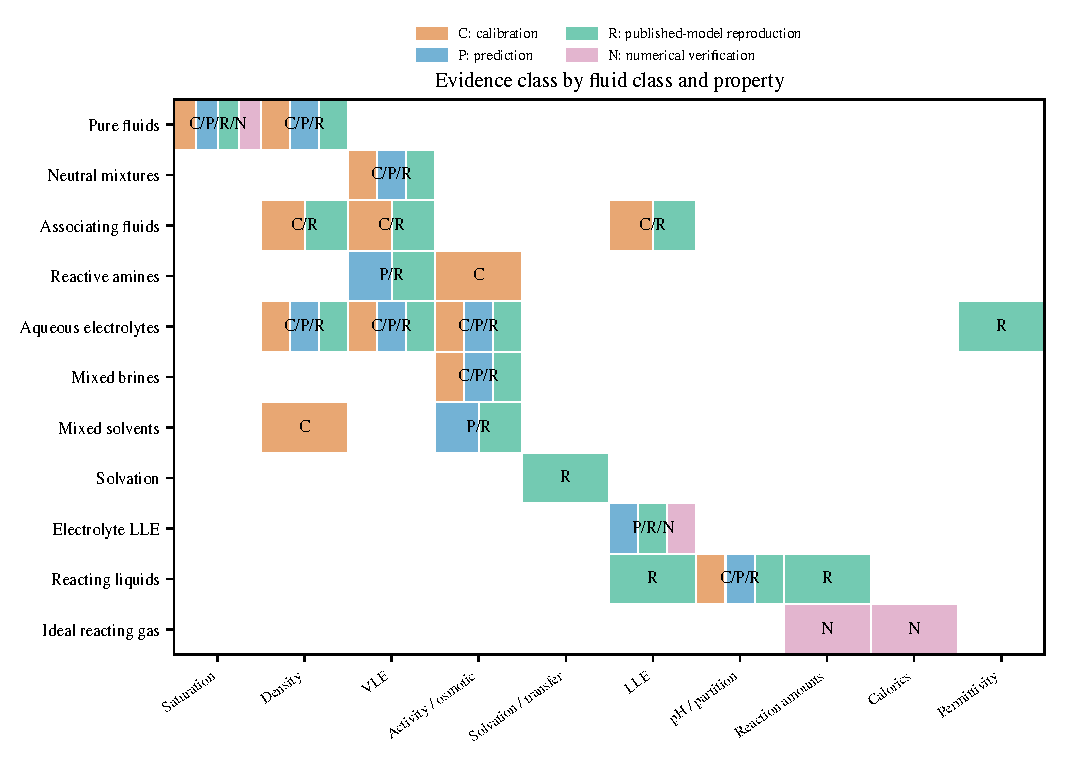
\includegraphics[width=0.94\linewidth]{F7-coverage}
\caption{The comparisons cover different physical quantities and evidence classes.
Calibration, prediction, published-model reproduction and numerical verification are distinguished, including split cells where more than one class applies.
Blank cells have no comparison in this work, and the map gives neither an accuracy ranking nor a count of independent datasets.
The per-population conditions, parameters and errors are given in Table~\ref{tab:physical-summary} and the complete Supporting Information table.}
\label{fig:coverage}
\end{figure}

% P:physical-02
For positive properties, the average absolute relative deviation is
\begin{equation}
\mathrm{AARD}=\frac{100}{n}\sum_{k=1}^{n}\left|\frac{y_k^{\mathrm{model}}}{y_k^{\mathrm{ref}}}-1\right|.
\label{eq:aard}
\end{equation}
Absolute mole-fraction and pH errors instead use the mean absolute error, and dimensional residuals or dimensionless coefficients can be summarized by a root-mean-square difference.
The table names the metric and unit because a pressure percentage, a pH-unit difference and an osmotic-coefficient residual cannot share a common accuracy scale.
Unavailable predictions remain identified, with statistics taken over the available comparisons rather than assigning a fictitious value to a failed solve.
Counts of repeated parameter variants or thermodynamically linked coordinates do not increase the number of independent measurements.

% P:physical-02b
Table~\ref{tab:physical-summary} gives the result by fluid class, and the subsections below explain each entry.
With published parameters, pure-fluid saturation pressures and liquid densities deviate from measurements or reference correlations by 0.281--2.70\,\% on average, and the zero-interaction methane/ethane prediction places both phase compositions within 0.008 mole fraction on average.
For aqueous 1:1 salts at 298.15~K the osmotic and mean ionic activity coefficients deviate by 1.72\,\% and 4.36\,\% from evaluated data that overlap the original parameter fit, and salted water/ethanol/isobutanol tie lines computed with the source parameters differ from the measurements by a mean 0.0111 mole fraction.
Accuracy is lost where parameters are carried beyond the data they were fitted to: unchanged published parameters fail every comparison range for NaCl--MgCl$_2$ and NaCl--CaCl$_2$ brines, NaCl activity coefficients deviate more in ethanol-rich than in water-rich solvents, the acetic acid partition coefficient deviates by 47.8\,\% although the aqueous pH is predicted within 0.146 unit, and MDEA parameters fitted to osmotic coefficients give total pressures with 96.2\,\% and 89.6\,\% AARD.
Refitting recovers a description within the fitted domain: a joint chloride fit predicts two withheld mixed-brine sources with RMS residuals of 0.00825 in osmotic coefficient and 0.00121 in water activity.
Section~\ref{sec:verification} shows that independent codes with matched models reproduce the package's state values to better than $10^{-8}$, so deviations of the size reported here belong to the model and its parameters, not to the numerical solution.



\begin{table}[pos=htbp]
\centering\footnotesize
\caption{Representative populations from the full comparison table. $N$ counts the displayed source rows; the methane/ethane comparison includes one unavailable state, and each aqueous 1:1-salt population includes 23 unavailable LiI rows. Their error means use 16 and 184 available comparisons, respectively. PRED denotes fixed-parameter prediction, CAL calibration and REPRO published-model reproduction. Original fitting overlap can remain unknown for inherited parameters. Pressure ranges are reference values; ``sat.'' denotes saturation with no separately reported density-row pressure.}
\label{tab:physical-summary}
\begin{tabularx}{\linewidth}{@{}p{0.19\linewidth}p{0.13\linewidth}p{0.13\linewidth}rX@{}}
\toprule
System / property & $T$/K & $P$/MPa & $N$ & Parameter role; error metric and value \\
\midrule
Propane / $P_{\rm sat}$ & 110--340 & $6\times10^{-7}$--2.43 & 24 & Gross--Sadowski; PRED, AARD 2.70\,\% \\
Propane / $\rho_L$ & 90--340 & sat. & 27 & Same; PRED, AARD 0.305\,\% \\
Propane / $\rho_V$ & 230--340 & sat. & 12 & Same; PRED, AARD 1.52\,\% \\
\ce{CO2} / $P_{\rm sat}$ & 220--300 & 0.599--6.71 & 17 & Gross quadrupolar; REPRO against reference equation, AARD 0.421\,\% \\
Benzene / $P_{\rm sat}$ & 290--540 & 0.00856--3.71 & 26 & Gross quadrupolar; REPRO against correlation, AARD 0.281\,\% \\
Methane/ethane / $x_{\ce{CH4}}$ & 203.22--243.61 & 2.124--6.885 & 17 & $k_{ij}=0$; PRED, MAE 0.00789 \\
Methane/ethane / $y_{\ce{CH4}}$ & 203.22--243.61 & 2.124--6.885 & 17 & $k_{ij}=0$; PRED, MAE 0.00412 \\
\ce{CO2}/THF / $x_{\ce{CO2}}$ & 313.2--353.2 & 0.47--10.29 & 34 & Schick inherited fit; REPRO/physical comparison, AARD 6.94\,\% \\
Aqueous 1:1 salts / $\gamma_\pm$ & 298.15 & 0.101 & 207 & Figiel inherited fit overlap; CAL, AARD 4.36\,\% \\
Same / $\Phi$ & 298.15 & 0.101 & 207 & Same; CAL, AARD 1.72\,\% \\
Joint chloride fit / $\Phi$ & 298.15 & 0.1 & 443 & Fitted source families; CAL, RMS 0.00748 \\
NaCl/\ce{CaCl2} / $\Phi$ & 298.15 & 0.1 & 53 & Joint fit, withheld source; PRED, RMS 0.00825 \\
NaCl/\ce{MgCl2} / $a_w$ & 298.15 & 0.1 & 19 & Joint fit, withheld source; PRED, RMS 0.00121 \\
NaCl/ethanol--water / $\gamma_\pm$ & 298.15 & unreported & 123 & Fixed Figiel parameters; PRED, AARD 6.35\,\% \\
Acetic acid/water/toluene / pH & 298.15 & 0.1 & 19 & Ascani, no pH fit; PRED, MAE 0.146 pH unit \\
Same / acid partition & 298.15 & 0.1 & 19 & Acid--organic calibration family; CAL, AARD 47.8\,\% \\
MDEA/\ce{CO2} / $P$ & 303 & 0.92--2.45 & 3 & Osmotic-fit S0/S1; PRED, AARD 96.2/89.6\,\% \\
\bottomrule
\end{tabularx}
\end{table}

\subsection{Pure nonpolar, dipolar and quadrupolar fluids}
% P:physical-03
Propane saturation with the Gross--Sadowski parameters~\citep{Gross2001}, Table~2, is compared with the later measurements of Glos et al.~\citep{Glos2004} in Supporting Information Fig.~\ref{fig:si-F8-pure-fluids-1} and, beside the refit, in Fig.~\ref{fig:fits}.
Pressure, liquid density and vapor density have different temperature populations and therefore separate statistics.
The pressure AARD of 2.70\,\% is larger than the liquid-density AARD of 0.305\,\%, with low-temperature pressures contributing strongly to the relative-pressure statistic.
The liquid-density observations are not all accompanied by a separately tabulated pressure in the selected population, so the table describes them as saturated states rather than inventing a pressure range.
The source expanded uncertainties are retained in the figure; they are not replaced by the numerical pressure-closure criterion.
All twelve vapor-density predictions lie outside their supplied uncertainty intervals; the low-temperature pressure discrepancy at 110~K lies inside its much larger interval.
The two coldest states, 110 and 120~K, where the measured pressures are 0.6 and 3.2~Pa, contribute 2.27 of the 2.70 percentage points; on the 19 temperatures withheld from the fit of Section~\ref{sec:estimation}, the published parameters give 1.07\,\% and 0.228\,\%.

% P:physical-04
The larger nonpolar catalogue contains one saturation calculation for each of 78 compounds from Gross and Sadowski~\citep{Gross2001}.
It establishes calculation breadth only: those catalogue states have no measured references from which to compute a 78-compound validation statistic.
Sparse source comparisons for methane, propylene, toluene and diethyl ether add liquid-density observations and paper-model samples in the Supporting Information.
At the coldest diethyl ether state the density misses the pressure-closure criterion, and at the coldest propylene state no density is returned; both states are marked and neither supports an accuracy statement.
The deviations that Gross and Sadowski report over their whole fitting datasets cannot be recomputed, because those observations are not available.

% P:physical-05
Dipolar acetone, dimethyl ether, diethyl ether and dimethyl sulfoxide test the optional Gross--Vrabec contribution~\citep{Gross2006} (Fig.~\ref{fig:pure-data}).
Published polar parameters, polar refits and nonpolar refits are distinct models in the full gallery.
Alternating training and withheld temperatures apply to the local refits.
The references for acetone, dimethyl ether and diethyl ether are the reference equations of state of Lemmon and Span~\citep{lemmonShortFundamentalEquations2006}, Wu et al.~\citep{wuEquationStateThermodynamic2011} and Thol et al.~\citep{tholNewFunctionalForm2014}, evaluated with CoolProp~8.0.0~\citep{bellPurePseudopureFluid2014}; they may share experimental data with the original published fit.
For acetone, the polar refit gives withheld pressure and liquid-density AARDs of 1.30\,\% and 0.669\,\%, compared with 0.936\,\% and 2.43\,\% for the nonpolar refit.
The example shows a property tradeoff: a smaller pressure error alone does not rank the overall formulation.
Because each formulation has its own fitted parameters, the difference cannot be attributed solely to switching on a dipole term at fixed parameters.
The DMSO measurements~\citep{Fulem2011,DePablo2018,Zhang2013,Paknejad2019} provide a separate source role and are not pooled with the evaluated reference equations as equivalent independent experiments.

\begin{figure}[pos=H]
\centering
\includegraphics[page=4,width=0.94\linewidth]{F8-pure-fluids}
\caption{Saturation pressure and liquid density of acetone, diethyl ether, dimethyl ether and dimethyl sulfoxide with the published polar parameters of Gross and Vrabec and with local polar and nonpolar refits~\citep{Gross2006}.
The refits use alternating training and withheld temperatures; references are reference equations of state for the first three fluids and measurements for dimethyl sulfoxide~\citep{lemmonShortFundamentalEquations2006,wuEquationStateThermodynamic2011,tholNewFunctionalForm2014,Fulem2011,DePablo2018,Zhang2013,Paknejad2019}.
Propane against the Glos measurements is in Fig.~\ref{fig:fits} and, with vapor densities, in the Supporting Information.}
\label{fig:pure-data}
\end{figure}

\begin{figure}[pos=H]
\centering
\includegraphics[page=5,width=0.94\linewidth]{F8-pure-fluids}
\par\small Figure~\ref{fig:pure-data} (continued).
\end{figure}

% P:physical-06
The quadrupolar parameters of Gross~\citep{grossEquationofstateContributionPolar2005}, Table~A1, are evaluated for carbon dioxide and benzene.
Their saturation-pressure AARDs are 0.421\,\% and 0.281\,\%, respectively, against the reference equation of Span and Wagner for carbon dioxide~\citep{spanNewEquationState1996}, evaluated with Clapeyron.jl, and a benzene vapor-pressure correlation.
These comparisons are identified as published-model reproduction against evaluated references.
They are useful tests of the selected model's pressure behavior over the displayed ranges, but they do not recover the original experimental fitting membership.
The benzene reference uses a DIPPR-101-form correlation whose coefficient attribution to the original compilation is unverified.
The nonpolar curves use their own parameters and therefore do not measure an isolated quadrupole correction.



\subsection{Neutral and polar mixture phase equilibria}
% P:physical-07
The methane/ethane comparison uses May et al.~\citep{May2015}, Table~5, with the Gross--Sadowski pure parameters and $k_{ij}=0$.
The measured liquid and vapor compositions define the physical references, while midpoint feeds are calculation declarations rather than measured feed inventories.
Sixteen of the 17 states return phase compositions and one is unavailable; two liquid and two vapor methane fractions lie outside three combined standard uncertainties of the measurement.
The available liquid and vapor methane fractions have MAEs of 0.00789 and 0.00412 over the displayed temperature and pressure range.
This is a fixed-parameter binary prediction, with no interaction fitted to this comparison (Supporting Information Fig.~\ref{fig:si-F9-neutral-mixtures-1}).

% P:physical-08
Acetone/$n$-pentane observations of Campbell et al.~\citep{Campbell1986}, Table~I, supply a stronger test of the distinction between calibration and temperature transfer.
The binary interaction is fitted at 372.7~K and then used at 397.7 and 422.6~K (Fig.~\ref{fig:mixture-data}).
At the withheld temperatures, the polar fitted model gives pressure AARDs of 1.55\,\% and 1.79\,\%, compared with 10.7\,\% and 8.70\,\% for its zero-interaction declaration.
The corresponding nonpolar fitted model gives 2.88\,\% and 2.81\,\%.
A Margules comparison is fitted independently at each isotherm, so its smaller residual cannot be interpreted as the same withheld-temperature prediction.
The observed improvement establishes transfer for these temperatures and compositions, without claiming a general advantage of a polar model for all mixtures.

\begin{figure}[pos=H]
\centering
\includegraphics[page=2,width=0.96\linewidth,height=0.6\textheight,keepaspectratio]{F9-neutral-mixtures}
\caption{Acetone/$n$-pentane bubble pressure and vapor composition against the measurements of Campbell et al.~\citep{Campbell1986}.
The binary interaction is fitted at 372.7~K (top row, calibration) and used unchanged at 397.7 and 422.6~K (lower rows, prediction), for the polar and nonpolar models; the zero-interaction polar model and a Margules correlation fitted separately at each temperature are shown for scale.
The methane/ethane zero-interaction prediction is in Supporting Information Fig.~\ref{fig:si-F9-neutral-mixtures-1}.}
\label{fig:mixture-data}
\end{figure}

% P:physical-09
Carbon dioxide/THF uses the fixed published parameters of Schick et al.~\citep{Schick2023}, Tables~1 and~6 and Supporting Information S3, against their tabulated experimental and model values.
The 34 liquid carbon-dioxide fractions span 313.2--353.2~K and 0.47--10.29~MPa, with an experimental AARD of 6.94\,\%.
Only five of the 34 calculated fractions reproduce the printed paper-model values; the remaining 29 discrepancies have no established source-side cause.
All 34 experimental comparisons lie outside the retained printed-resolution criterion, which is not a measurement-uncertainty interval.
The published model values remain a separate series in the full mixture gallery.
Agreement with those calculated values tests the translation of the paper model; comparison with the observations tests the model's solubility description and inherits its source fitting history.
The Gross--Sadowski binary gallery adds hydrocarbon and carbon-dioxide mixtures with figure-specific interactions~\citep{Gross2001}; the largest deviation from measurements among them is 15.8\,\% AARD for four carbon dioxide/$n$-decane bubble pressures.
Those sparse model and experimental references remain separate, so reproduction of a source curve does not become an extra measured dataset.



\subsection{Associating pure fluids and mixtures}
% P:physical-10
Association changes the relative preference for hydrogen-bonding and hydrocarbon-rich phases, and its parameters must be evaluated together with the site topology.
The Gross--Sadowski associating comparisons~\citep{Gross2002} include saturated alcohol densities and bubble/dew behavior of alcohol/hydrocarbon and alcohol/aromatic mixtures.
Figure~\ref{fig:association-data} shows the water/1-pentanol phase-temperature and liquid-composition branches, with the other binary systems in the full gallery.
Measured markers, supplemental observations and digitized source-model curves retain separate symbols and comparison rows.
These are mainly calibration-related physical comparisons with inherited parameters; exact observation overlap is incomplete.

\begin{figure}[pos=H]
\centering
\includegraphics[page=3,width=0.94\linewidth]{F10-associating}
\caption{Water/1-pentanol at 0.1013~MPa with the Gross--Sadowski parameters and the source's binary interaction~\citep{Gross2002}: phase temperatures against the water mole fraction (left) and the compositions of the two liquids against temperature (right).
Open symbols are measurements and crosses this package's values; the star marks the calculated three-phase temperature.
The parameters were fitted to data of this kind, so the comparison is calibration-related.}
\label{fig:association-data}
\end{figure}

% P:physical-11
Pure-fluid liquid and vapor statistics remain separate because mixing the branches would obscure both the density scale and the error.
For example, the package reproduces the published 1-pentanol saturated-liquid curve within 0.362~kg/m$^3$ MAE between 280 and 560~K, but deviates by 6.04\,\% AARD from the measured liquid densities, which extend to 585~K, beyond the end of the published curve.
The measured saturated-vapor densities of methanol deviate by 32.9\,\% AARD over six states, the largest associating-fluid deviation in the full table.
Agreement with a published model line therefore does not establish agreement with the measurements shown beside it.
The same distinction matters for isobutane/methanol and the propanol/benzene systems, whose source-model and measured pressure samples have different populations.
The complete comparison table preserves each one rather than replacing them by an aggregate associating-fluid accuracy.

% P:physical-12
Water/1-pentanol extends the comparison to liquid--liquid--vapor behavior at 0.1013~MPa.
The selected bubble-temperature observations have a 4.46~K MAE, while the computed three-phase temperature differs from the sampled source trace by 0.661~K.
The full gallery shows the phase-temperature and liquid-composition branches and identifies the single calculated three-phase state.
Default starts fail for some source dew declarations; explicit starts recover the intended branches in the selected comparison.
That result concerns branch selection and initialization, rather than proving that the source phase diagram has been completely discovered.



\subsection{Aqueous single electrolytes and permittivity}
% P:physical-13
Mean ionic activity and practical osmotic coefficients test related but different derivatives of the electrolyte free energy.
The Hamer--Wu evaluated coefficients~\citep{HamerWu1972}, computed with the fixed Figiel parameters~\citep{Figiel2025}, cover lithium, sodium and potassium halides at 298.15~K.
Each observable has 207 source values, of which 184 have available predictions and 23 LiI values are unavailable.
The AARDs over the 184 available comparisons are 4.36\,\% for ionic activity and 1.72\,\% for osmotic coefficient.
Figure~\ref{fig:aqueous-data} shows both observables.
The original fitting overlap is only partly resolved, so the figure classifies them as calibration-related comparisons.
LiI remains unavailable because the required lithium/iodide source interaction is not supplied.
Omitting it from the error mean does not establish its physical accuracy.

\begin{figure}[pos=H]
\centering
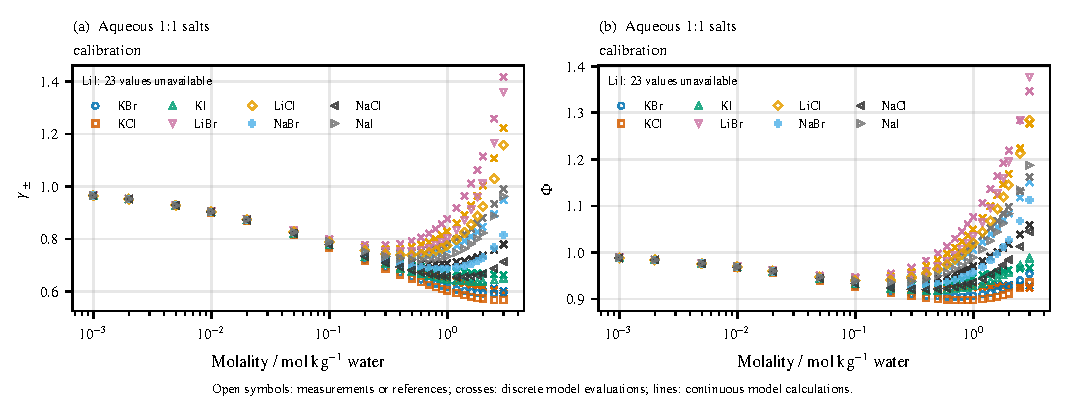
\includegraphics[page=1,width=0.94\linewidth]{F11-aqueous-electrolytes}
\caption{Mean ionic activity coefficients (left) and practical osmotic coefficients (right) of eight lithium, sodium and potassium halides at 298.15~K against the evaluated values of Hamer and Wu, computed with the Figiel parameters~\citep{HamerWu1972,Figiel2025}.
Open symbols are the evaluated values and crosses this package's values; LiI is not computed because the source supplies no lithium/iodide interaction.
The parameters were fitted partly to these data, so the comparison is calibration-related.
NaCl permittivity alternatives and the Held salt series are in the Supporting Information.}
\label{fig:aqueous-data}
\end{figure}

% P:physical-14
Held et al.~\citep{Held2008} broaden the properties to density, vapor pressure, water activity and mean ionic activity across 19 salts and 45 source series.
The full gallery displays every series with its source-line and measured-marker roles.
Unresolved neighboring source curves and disagreements remain visible, and the reconstruction is partial.
A pooled percentage over sampled correlated pixels would not be an experimental accuracy statistic, so none is given.
The separate Held osmotic comparisons~\citep{Held2014} at 273.15 and 298.15~K add a bounded temperature comparison, with the inferred diameter convention described in the Supporting Information.
They do not establish general temperature transfer for all electrolytes.

% P:physical-15
The NaCl permittivity comparison in the full aqueous gallery links activity accuracy to another physical quantity.
With the Figiel parameters and ion-suppression relation unchanged, the low- and higher-molality activity AARDs are 4.39\,\% and 5.35\,\%.
Refitting one shared water--ion interaction to the 21 activity observations at or below 2~mol/kg gives 0.666\,\% in that fitted population but 18.2\,\% over the eight higher-molality observations.
The density--temperature and dipolar-perturbation alternatives give withheld AARDs of 13.8\,\% and 16.7\,\%, yet miss much of the observed dielectric decrement.
Their relative-permittivity AARDs are 21.0\,\% and 23.5\,\%, compared with 7.27\,\% for ion suppression.
A more favorable activity extrapolation therefore does not by itself justify adopting a permittivity relation.
The alternative forms retain ion and Born parameters fitted with another relation, while primary-table lineage and pointwise measurement uncertainty remain unverified for this dielectric population.



\subsection{Mixed brines: failed transfer and a conditional refit}
% P:physical-16
A binary-salt parameter fit does not automatically constrain the cross-composition behavior of a mixed brine.
At 298.15~K and 100~kPa, the unchanged Held and Figiel parameters~\citep{Held2014,Figiel2025} fail the comparison limit in every source and ionic-strength range of the NaCl--MgCl$_2$ and NaCl--CaCl$_2$ water-property comparison~\citep{rardIsopiesticDeterminationOsmotic1987a,robinsonPropertiesAqueousMixtures1966,dinaneWaterActivitiesOsmotic2003a}.
Figure~\ref{fig:brine-data} compares residuals of the practical osmotic coefficient for the isopiestic data and the water activity for the Dinane--Mounir data.
The failure applies to these published parameter sets; it does not show that the equations cannot describe mixed salts with other parameters.

\begin{figure}[pos=H]
\centering
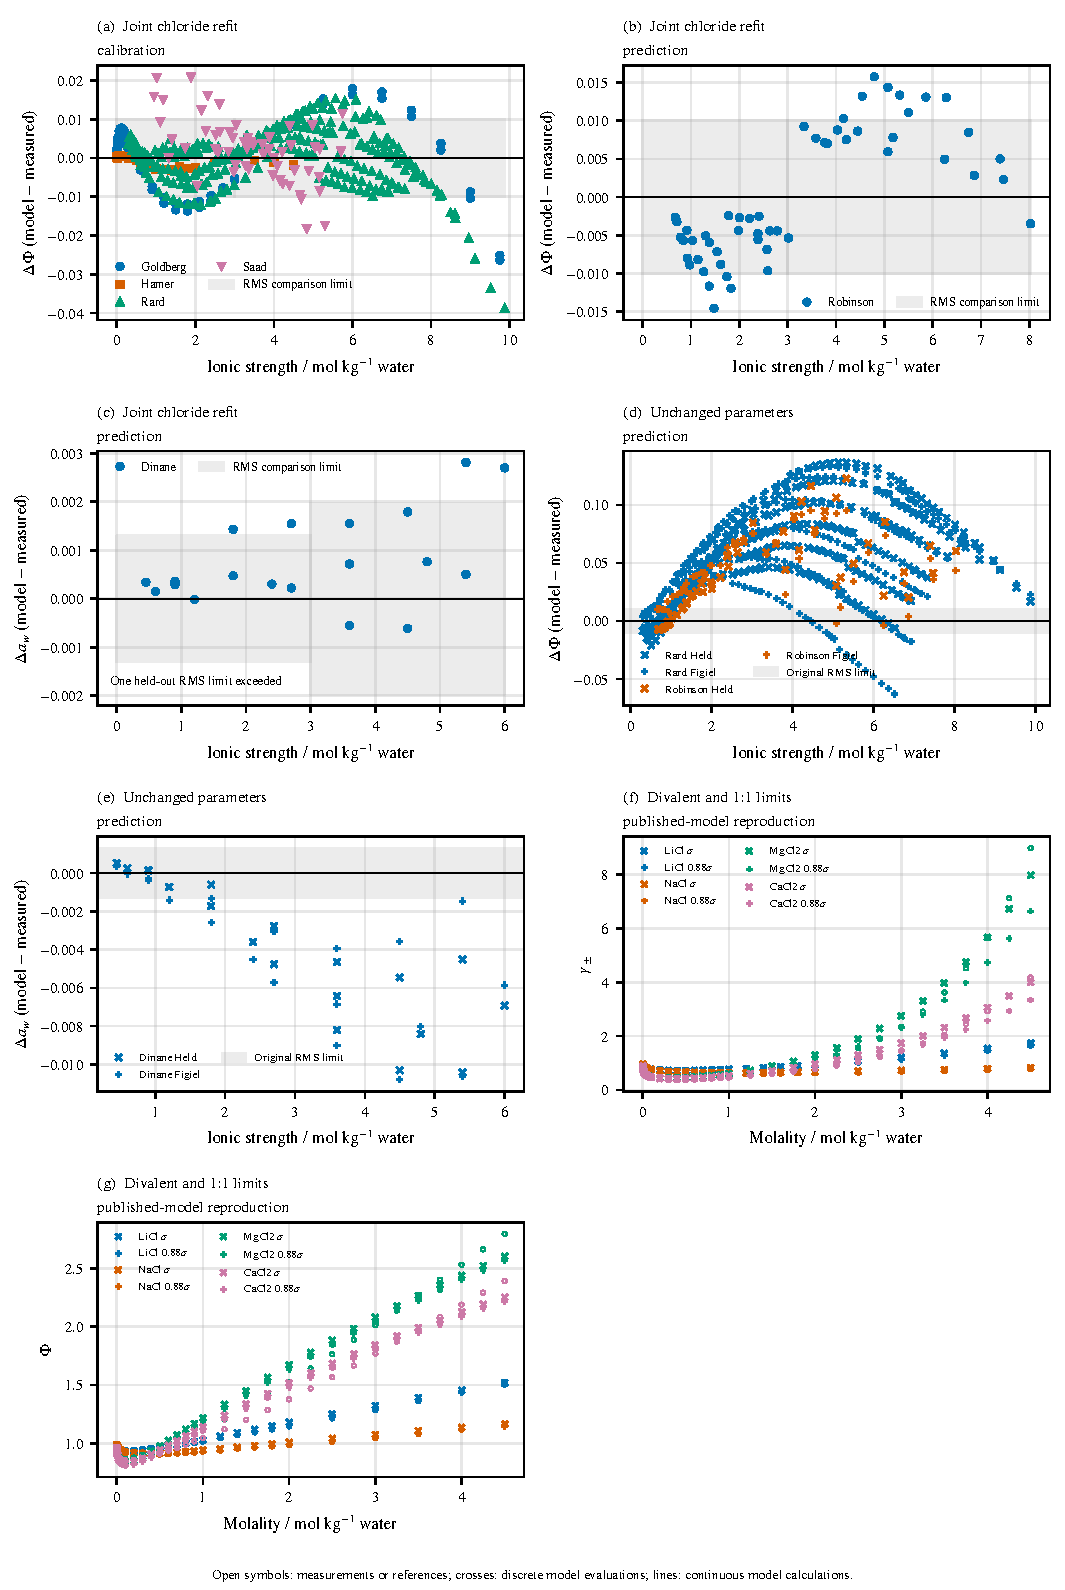
\includegraphics[width=0.91\linewidth,height=19cm,keepaspectratio]{F12-mixed-brines}
\caption{Residuals of mixed chloride brines at 298.15~K and 100~kPa against ionic strength.
Joint Figiel-form fit: (a) osmotic-coefficient training data, (b) withheld Robinson--Bower NaCl--CaCl$_2$ osmotic coefficients and (c) withheld Dinane--Mounir NaCl--MgCl$_2$ water activities.
Shaded bands in (a)--(e) show the corresponding RMS comparison limits, not pointwise measurement uncertainties; (c) uses the nominal source-agreement limit.
Unchanged published Held and Figiel parameters: (d) osmotic coefficients and (e) water activities of the same mixtures.
(f) Mean ionic activity and (g) osmotic coefficients of LiCl, NaCl, MgCl$_2$ and CaCl$_2$ with the Held strategy-2 parameters and the ion diameters $\sigma_i$ and $0.88\sigma_i$~\citep{Held2014}.}
\label{fig:brine-data}
\end{figure}

% P:physical-17
A joint Figiel-form fit adds binary NaCl, MgCl$_2$ and CaCl$_2$ osmotic data~\citep{HamerWu1972,goldbergEvaluatedActivityOsmotic1978}, Rard--Miller NaCl--MgCl$_2$ mixtures~\citep{rardIsopiesticDeterminationOsmotic1987a} and Saad NaCl--KCl--CaCl$_2$ mixtures~\citep{saadThermodynamicsMixedElectrolyte1980}, with the potassium parameters held fixed.
Its 443 training rows have RMS osmotic residual 0.00748.
The Rard--Miller data are calibration here, although they were predictions in the unchanged-parameter study.
Independent-source Robinson--Bower NaCl--CaCl$_2$~\citep{robinsonPropertiesAqueousMixtures1966} and Dinane--Mounir NaCl--MgCl$_2$~\citep{dinaneWaterActivitiesOsmotic2003a} mixtures supply the withheld data: RMS residuals are 0.00825 in osmotic coefficient and 0.00121 in water activity.
These values use the source data as printed.

% P:physical-18
Above an ionic strength of 3~mol/kg, the Rard--Miller training data, converted to water activity at the Dinane--Mounir compositions, differ from the Dinane--Mounir measurements by more than the original water-activity limit, so no model fitted to Rard--Miller can meet that limit.
After the fit, the limit for each Dinane--Mounir ionic-strength range was therefore set to the larger of the original limit and the disagreement between the two sources on the same rows, and applied to the existing fit without refitting.
To test the effect of rounding in the source tables, the comparison used the nominal data and 1466 perturbed versions that shift printed values by half a unit in their last printed digit.
The fit meets every withheld limit in 1466 of them; in the remaining one, which lowers every printed Dinane--Mounir value, the water-activity RMS for $I\le3$~mol/kg water is 0.001376 against a limit of 0.001352.
These perturbed data sets are sensitivity cases, not a probability distribution or new measurements.
The result supports a conditional description of the selected held-out mixtures at ionic strengths $I=0.45$--$8.03$~mol/kg water, with that explicit exception.
Above the held-out range, only training and reference checks are available: the magnesium-rich Rard--Miller training maximum $|\Delta\Phi|$ is 0.0388, and the separate pure-MgCl$_2$ reference check gives RMS 0.0289 and maximum 0.0376, exceeding the corresponding osmotic limits of 0.01 and 0.03.
The result does not demonstrate arbitrary simultaneous sodium/magnesium/calcium mixture accuracy or single-ion activities.
The corresponding Held-form fit is not offered as a mixed-brine description.

% P:physical-19
Divalent-salt comparisons also show why a diameter convention cannot be treated as a cosmetic input.
The paired Held strategy-2 screening declarations use $\sigma_i$ or $0.88\sigma_i$ and retain different errors for LiCl, NaCl, MgCl$_2$ and CaCl$_2$.
The full comparison reaches maximum absolute decadic errors of 0.131 for ionic activity and 0.0460 for osmotic coefficient over the paired population.
These maxima combine declared variants and are not an accuracy estimate for one adopted parameter set.
The divalent failures remain visible even where the monovalent coefficients are well represented.



\subsection{Mixed solvents, alcohol salts and solvation energies}
% P:physical-20
Solvent composition changes both the neutral mixture and the electrostatic environment of an ion.
Voltage-derived NaCl activity coefficients reported by Esteso et al.~\citep{Esteso1989}, Table~I, test fixed Figiel mixed-solvent parameters at 298.15~K across ethanol--water compositions.
The 123 comparisons give a pooled AARD of 6.35\,\%, with larger discrepancies in ethanol-rich mixtures than in the water-rich part of the population, although the trend is not monotonic.
Figure~\ref{fig:solvent-data} displays the composition dependence rather than replacing it by the pooled value.
The printed-digit comparison criterion is not a complete experimental uncertainty and supplies no claim that all excluded pointwise agreements are experimentally resolved failures.

\begin{figure}[pos=H]
\centering
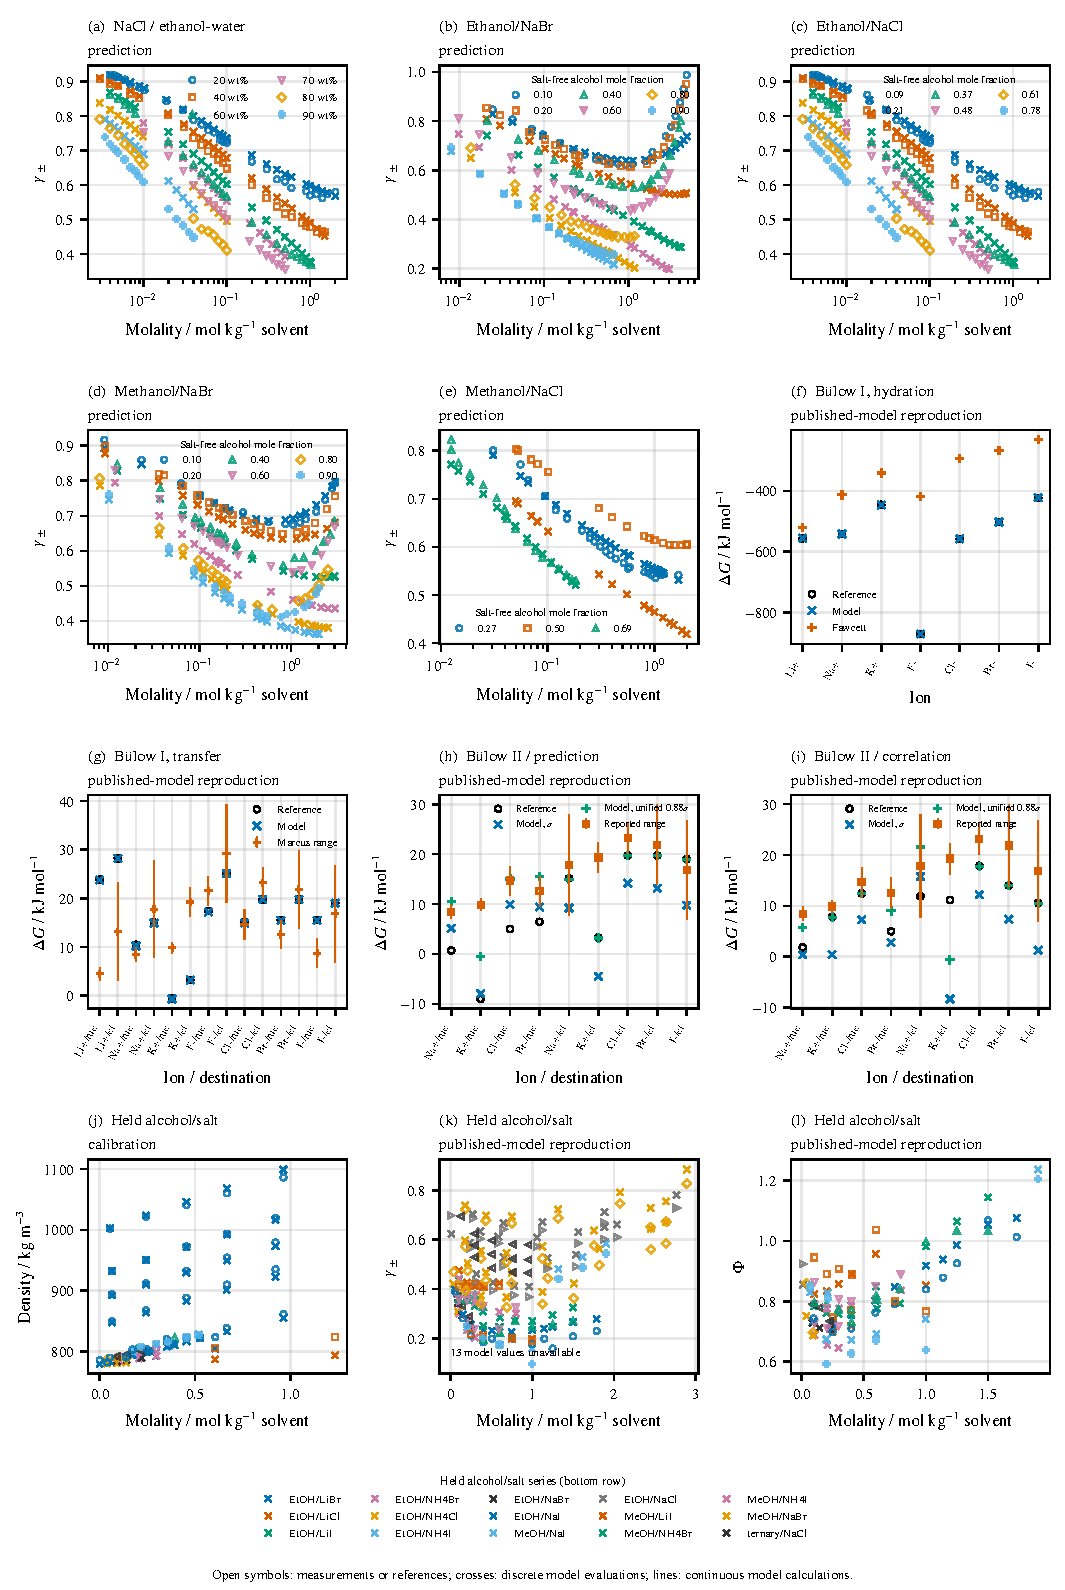
\includegraphics[width=0.91\linewidth,height=19cm,keepaspectratio]{F13-mixed-solvents-solvation}
\caption{Mixed-solvent activity, single-ion solvation and alcohol/salt properties constrain different parts of an electrolyte model~\citep{Esteso1989,Figiel2025,Bulow2020,Bulow2021,Held2012}.
Panels distinguish fixed-parameter prediction, calibration and published-model reproduction.
The Esteso and Figiel ethanol--NaCl observations overlap; reference ranges for single ions retain their conventions, and source-model bars remain separate from physical reference values.
}
\label{fig:solvent-data}
\end{figure}

% P:physical-21
The Figiel water--methanol and water--ethanol comparisons~\citep{Figiel2025} are fixed-parameter mixture predictions for NaCl and NaBr.
The NaBr parameters inherit pure-solvent activity fitting, so this classification does not establish independence from model development.
The four selected interior populations have dimensionless coefficient RMS differences from 0.0435 to 0.153.
Their primary-source lineage and measurement uncertainty are incomplete, and no independent-validation threshold is supplied.
The ethanol--NaCl population duplicates the Esteso observations, so displaying it under another model comparison does not add an independent dataset.
Excluded endpoints and the source limitations are preserved in the full table.

% P:physical-22
Ion hydration and solvent-transfer energies add another observable family~\citep{Bulow2020,Bulow2021}.
The figures compare model bars separately from the conventional single-ion reference values and ranges.
They show which diameter interpretation reproduces the paper calculations and where the transfer differs from those references.
Single-ion free energies depend on the adopted convention and are not convention-free direct measurements.
Agreement within the reading interval of a published model bar therefore tests model translation, not an independent hydration experiment.
The inferred $0.88\sigma_i$ diameter and the separation of correlated and predicted transfer populations remain explicit.

% P:physical-23
Alcohol/salt data from Held et al.~\citep{Held2012} add solution density, osmotic coefficient and derived ionic activity in methanol and ethanol.
The source parameters are solvent-specific and fitted to density and osmotic observations.
Derived ionic activities do not constitute an independent second osmometric experiment.
The direct tabulated comparisons miss the adopted printed-resolution criteria, while agreement with sampled source curves varies by property.
The source solvent-caption correction and the unresolved differences limit the interpretation to these declared calibration and reproduction comparisons.
They do not establish general salt transfer between water and alcohols.



\subsection{Electrolyte and reacting liquid splits}
% P:physical-24
The water/ethanol/isobutanol/NaCl comparison uses the Khudaida source parameters~\citep{Khudaida2026} for eight measured tie lines, solved at 293.15~K and 100~kPa with nominal 5~wt\% salt.
Each measured phase is expressed on a four-component formula basis, with NaCl counted as a formula unit rather than as two independent species fractions.
The mean absolute difference over the four coordinates of both phases is 0.0111 in mole fraction.
Figure~\ref{fig:reacting-data} shows the salt coordinates beside the solvent projection, preventing a favorable ternary projection from concealing salt-partition errors.
The adopted correlation-scale comparison is not agreement within measurement uncertainty, and the coordinate count is not a count of independent tie-line observations.
The manufactured feeds define the calculation without using measured endpoints as solver starts.

\begin{figure}[pos=H]
\centering
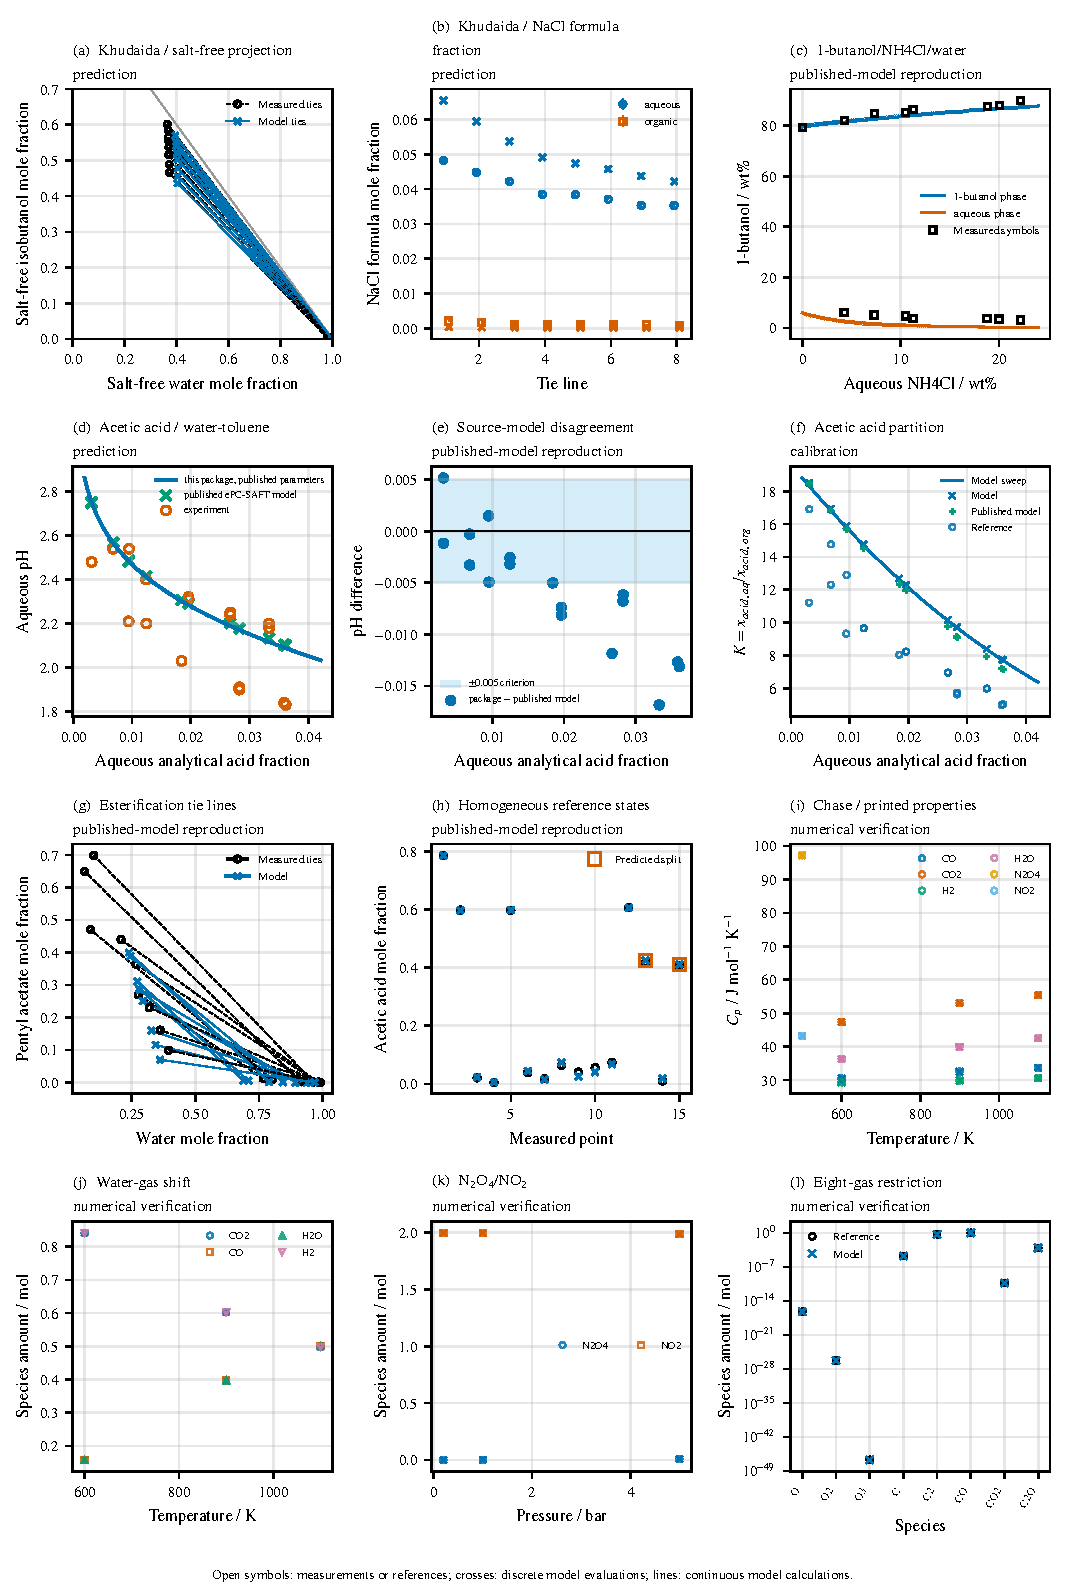
\includegraphics[width=0.91\linewidth,height=19cm,keepaspectratio]{F14-lle-reacting}
\caption{Liquid-split and reacting comparisons preserve the distinction between measured phases, source-model lines and numerical references~\citep{Khudaida2026,Held2014,Ascani2022pH,Ascani2023,Senina2022,Belov2023}.
The salted tie-line projection has a separate NaCl-coordinate panel; acid pH is paired with molecular partitioning; esterification retains incorrect phase counts.
The ideal-gas thermochemical and reaction-amount panels are numerical verification.
}
\label{fig:reacting-data}
\end{figure}

% P:physical-25
The 1-butanol/NH$_4$Cl/water comparison~\citep{Held2014} has a different reference role.
Its reference is a digitized published model line, not an additional set of measured tie lines.
The maximum selected butanol mass-percentage difference is 0.432 percentage point with the declared inferred ion-diameter convention.
That agreement establishes bounded reproduction of the calibrated source model.
The full table keeps this population separate from the measured Khudaida coordinates.

% P:physical-26
Acetic acid dissociation and water autoprotolysis coupled to water/toluene liquid splitting test reaction references and phase equilibrium together~\citep{Ascani2022pH}.
The aqueous pH predictions have MAE 0.146 pH unit at 19 measured compositions.
Only seven source-model pH values meet the separate 0.005-unit reproduction criterion, with maximum absolute difference 0.0169 pH unit.
The molecular-acid partition coefficient is $K=x_{\mathrm{acid,aq}}/x_{\mathrm{acid,org}}$, distinct from the reaction equilibrium constant.
It gives 47.8\,\% AARD against the measured partition population, whose acid--organic interaction belongs to a calibration family with unresolved exact overlap.
The pH and partition results therefore support different conclusions; a relatively close pH curve does not establish accurate distribution of acid between the liquids.
Organic trace-ion amounts and organic pH remain unresolved, and no charged phase-stability conclusion follows.

% P:physical-27
Reactive esterification adds acetic acid, 1-pentanol, pentyl acetate and water at 318.15~K~\citep{Ascani2023,Senina2022}.
The selected homogeneous and tie-line composition RMS differences are 0.00738 and 0.0829, respectively.
The reaction constant partly inherits calibration to the measured system, so these are published-model/calibration-related physical comparisons.
The wrong predicted phase counts for measured homogeneous points 13 and 15 remain in the interpretation.
Satisfying the reaction residual at a computed split does not correct a wrong phase count or make the tie-line error small.
The gas-reaction panels in the same gallery check ideal thermochemistry and equilibrium amounts against reference calculations~\citep{linstromNISTChemistryWebBook1997,Belov2023}; they are numerical verification and add no physical reacting-liquid validation.



\subsection{Reactive amines: calibration does not establish pressure accuracy}
% P:physical-28
The MDEA examples expose a substantial limit of transferring a fitted electrolyte description to reacting vapor--liquid equilibrium.
For the Wangler formulation~\citep{Wangler2018}, ten osmotic observations at 273 and 313~K determine a water--protonated-MDEA interaction under two declared ion-dispersion conventions, S0 and S1.
The calibrated osmotic AARDs are between 1.43\,\% and 2.65\,\% across temperature and convention.
The subsequent pressure comparison at 303~K and 60~wt\% MDEA was not used in that fit.
It gives 96.2\,\% and 89.6\,\% AARD for the fitted S0 and S1 variants at the three measured pressures.
Figure~\ref{fig:amine-data} shows both the fitted coefficients and failed pressure transfer.
The cause remains an unresolved model-reading or parameter-transfer discrepancy; this evidence does not establish a general defect of every MDEA formulation and supplies no MEA accuracy result.

\begin{figure}[pos=H]
\centering
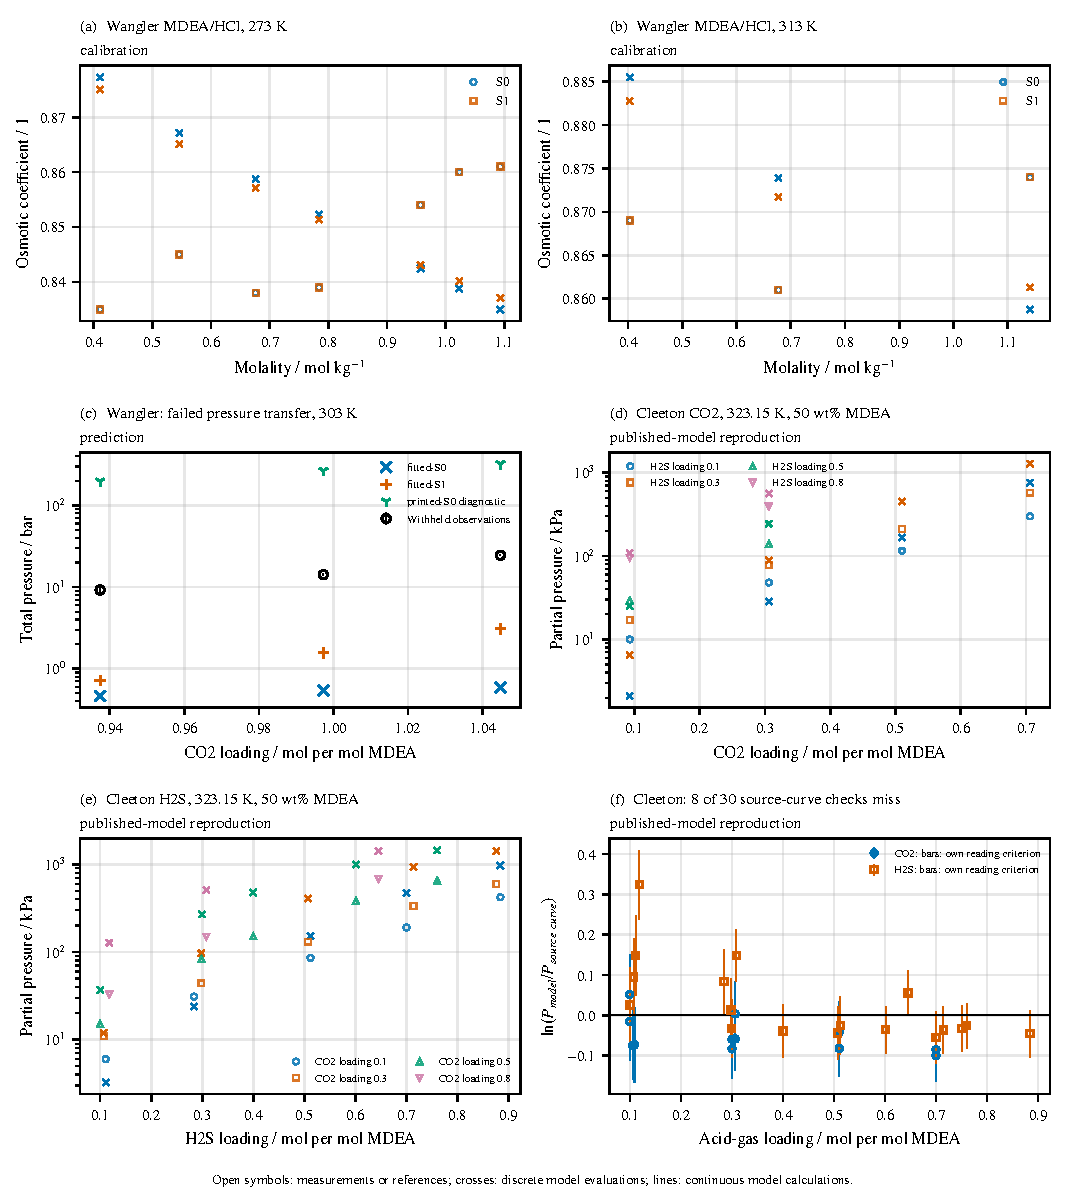
\includegraphics[width=0.92\linewidth,height=18cm,keepaspectratio]{F16-reactive-amines}
\caption{Reactive MDEA comparisons retain unsuccessful transfer~\citep{Wangler2018,Cleeton2020}.
The Wangler panels separate osmotic calibration from pressure prediction at withheld conditions.
The Cleeton panels separate measured partial-pressure comparisons from published-curve reproduction, including eight source-curve misses and the methane omission.
Grey markers (printed-S0) use the Wangler parameters as printed in the source and are shown as a diagnostic, not a fit.}
\label{fig:amine-data}
\end{figure}

% P:physical-29
The Cleeton comparison~\citep{Cleeton2020} recalculates competitive CO$_2$/H$_2$S absorption in 50~wt\% MDEA at 323.15~K with inherited source parameters and no refit to the selected partial pressures.
The primary published-curve reading meets its digitization criterion at 22 of 30 points, leaving eight curve misses.
Ordinary AARDs against the measured CO$_2$ and H$_2$S partial pressures are 64.4\,\% and 143.7\,\%.
These differ from a symmetric relative-deviation statistic, which gives less weight to large overprediction and cannot be reported under the same AARD definition.
The declaration omits methane present in the source record and uses the stated inferred ionic-diameter convention.
It is a bounded published-model replay with large physical discrepancies, rather than an absorption-prediction success.
